\documentclass{beamer}
\usetheme{Frankfurt}
\usecolortheme{seahorse}
\usefonttheme{serif}

\author{Mgr. Jiří Květoň}
\date{June 23, 2023}

\title{Analysis and Modelling of Non-linear Dynamical Systems in Astrophysics}
\subtitle{Multilayer Dripping Handrail Accretion Disk Model}

\usepackage[font=tiny,labelfont=bf,labelformat=empty]{caption}
\usepackage{amsmath,pgfpages}
\usepackage{derivative}
\usepackage[export]{adjustbox}

\makeatletter
\let\originalnote\note
\renewcommand<>\note[2][]{\ifmeasuring@\else\originalnote#3[#1]{#2}\fi}
\makeatother

\defbeamertemplate*{title page}{customized}[1][]{
    \begin{center}
        \usebeamerfont{title}\inserttitle\par

        \vspace{3mm}

        \scriptsize\itshape\insertsubtitle\par

        \bigskip

        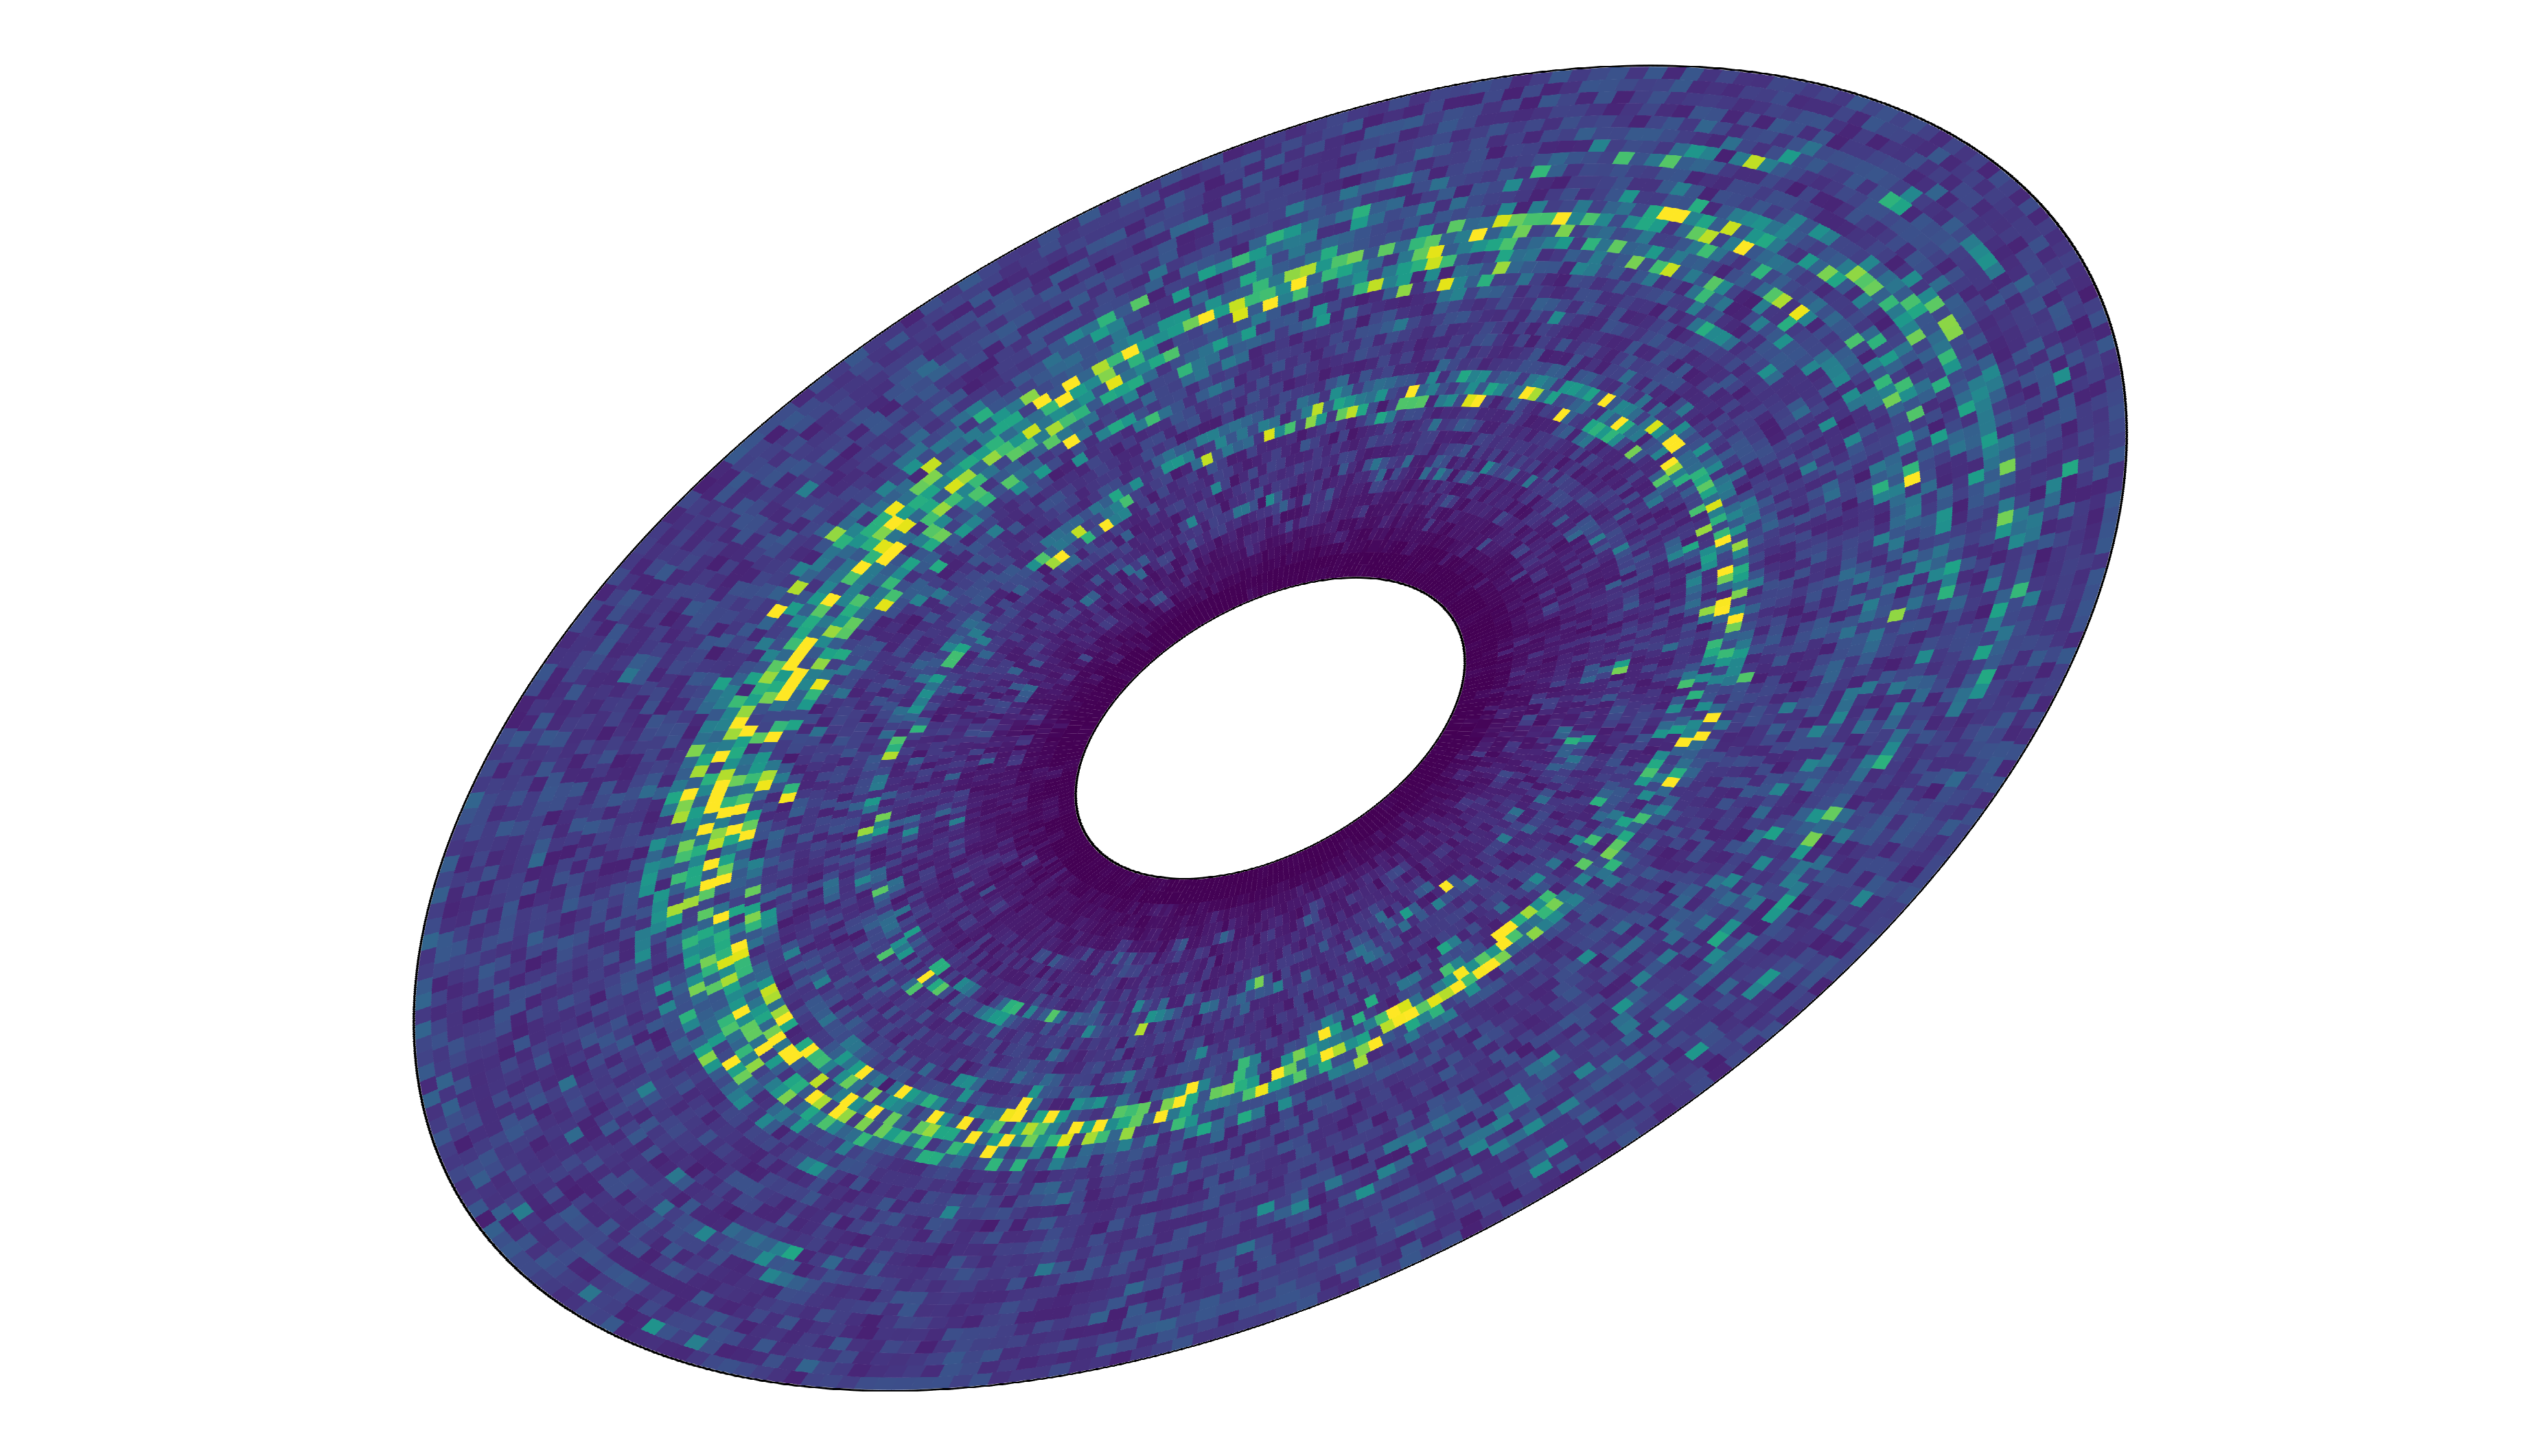
\includegraphics[height=.4\textheight]{img/cover.png}
        
        \bigskip

        \upshape\usebeamerfont{date}\insertauthor \hspace{30mm} \insertdate\par
    \end{center}
}

\begin{document}

\maketitle

%% Outline
% \setbeamertemplate{section in toc}[ball unnumbered]
% \begin{frame}{OUTLINE OF THE TALK}
    % \tableofcontents
% \end{frame}


%% Polulární uvod
\section{Motivation}
\begin{frame}
    \begin{center}
        \begin{figure}
            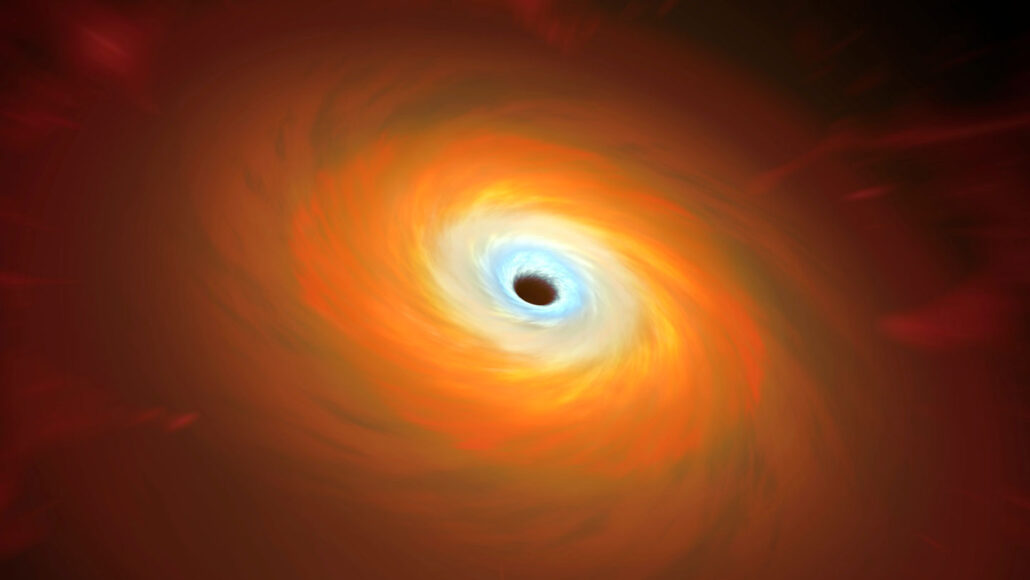
\includegraphics[width=1\textwidth]{img/disk_1.jpg}
            \caption{Taken from (Science Photo Library, Mark Garlic, 2023)}
        \end{figure}
    \end{center}
\end{frame}

\begin{frame}
    \begin{center}
        \begin{figure}
            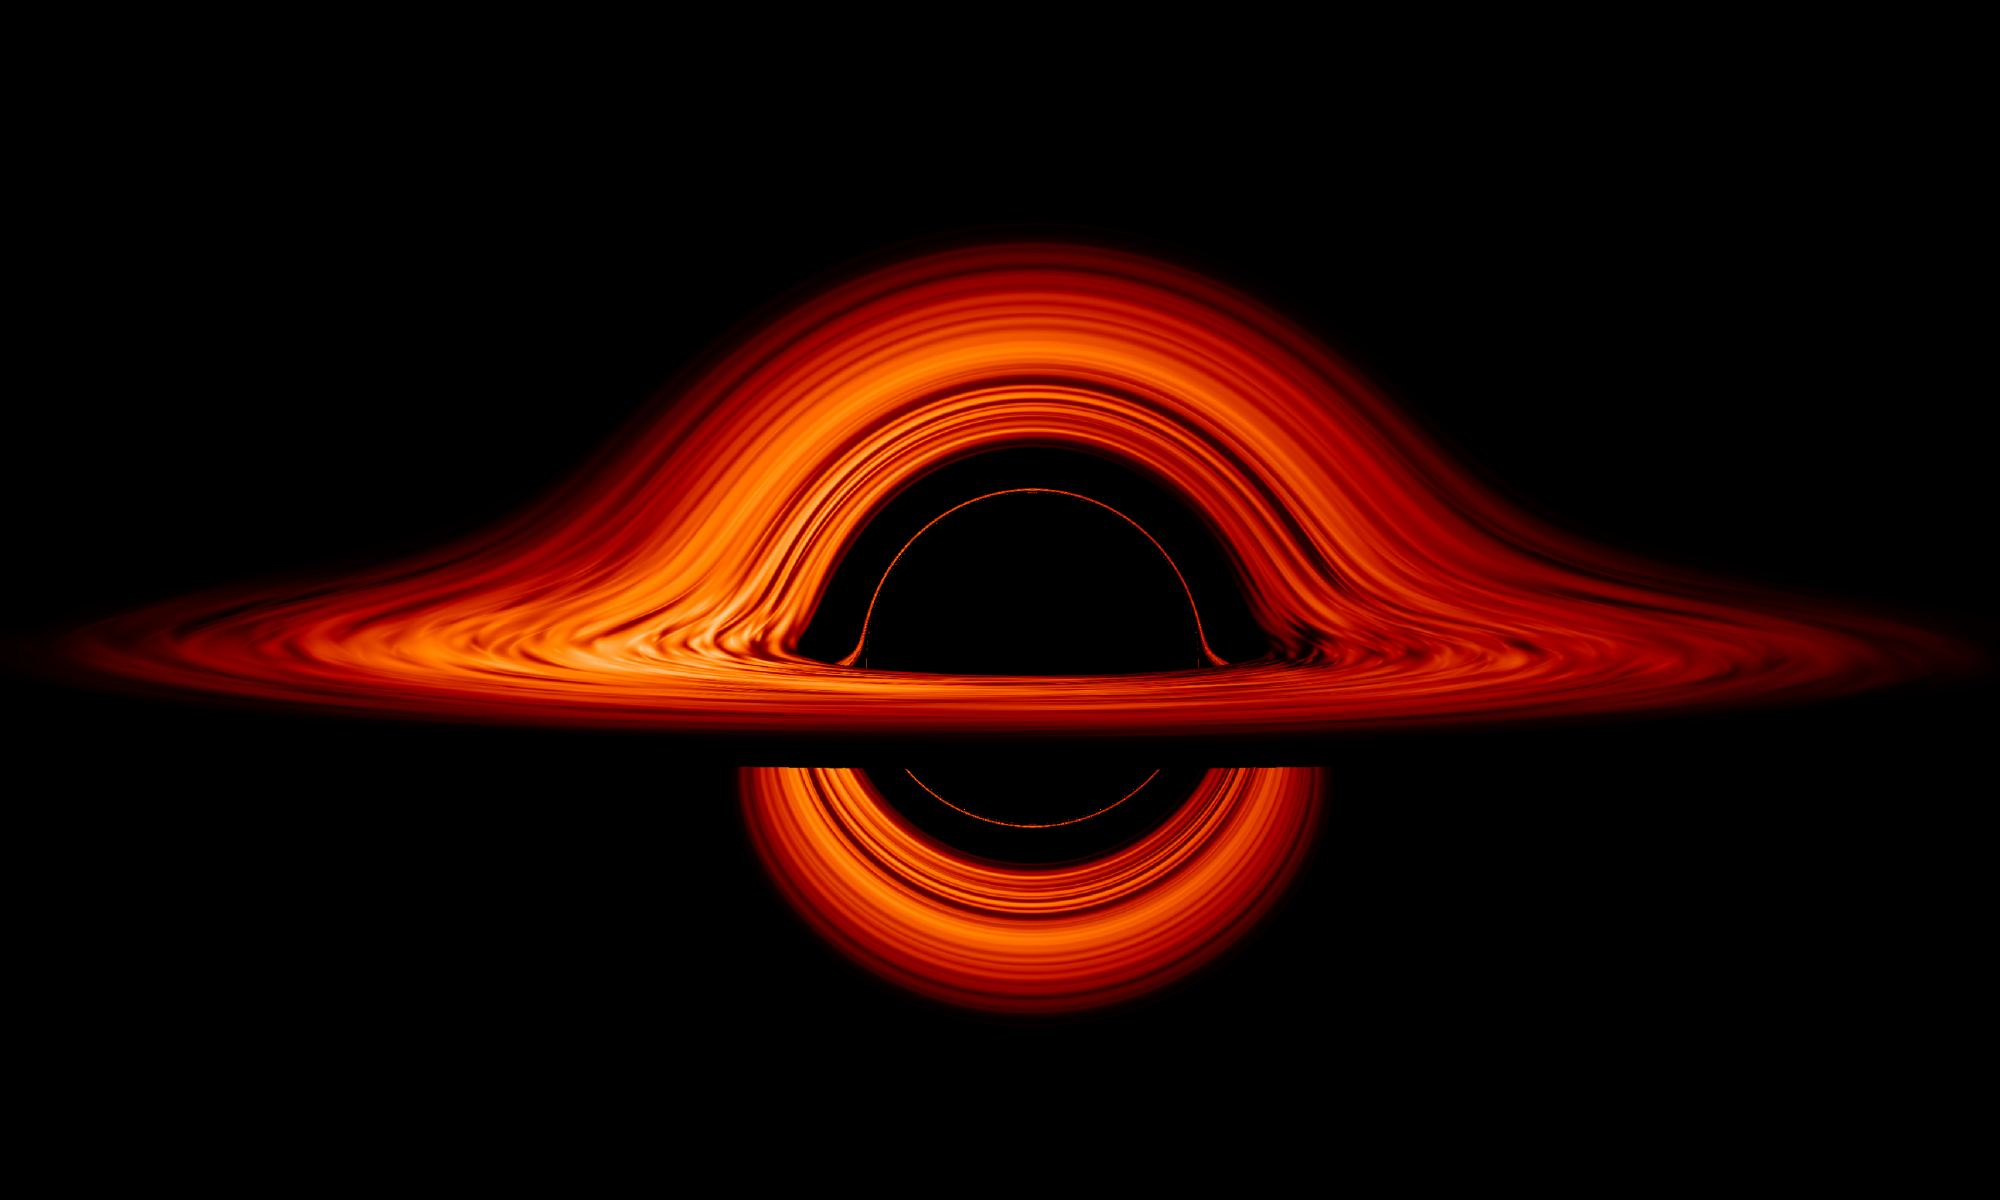
\includegraphics[width=1\textwidth]{../img/bh_warped.jpg}
            \caption{Taken from (NASA’s Goddard Space Flight Center, 2019)}
        \end{figure}
    \end{center}
\end{frame}

\begin{frame}
    \begin{center}
        \begin{figure}
            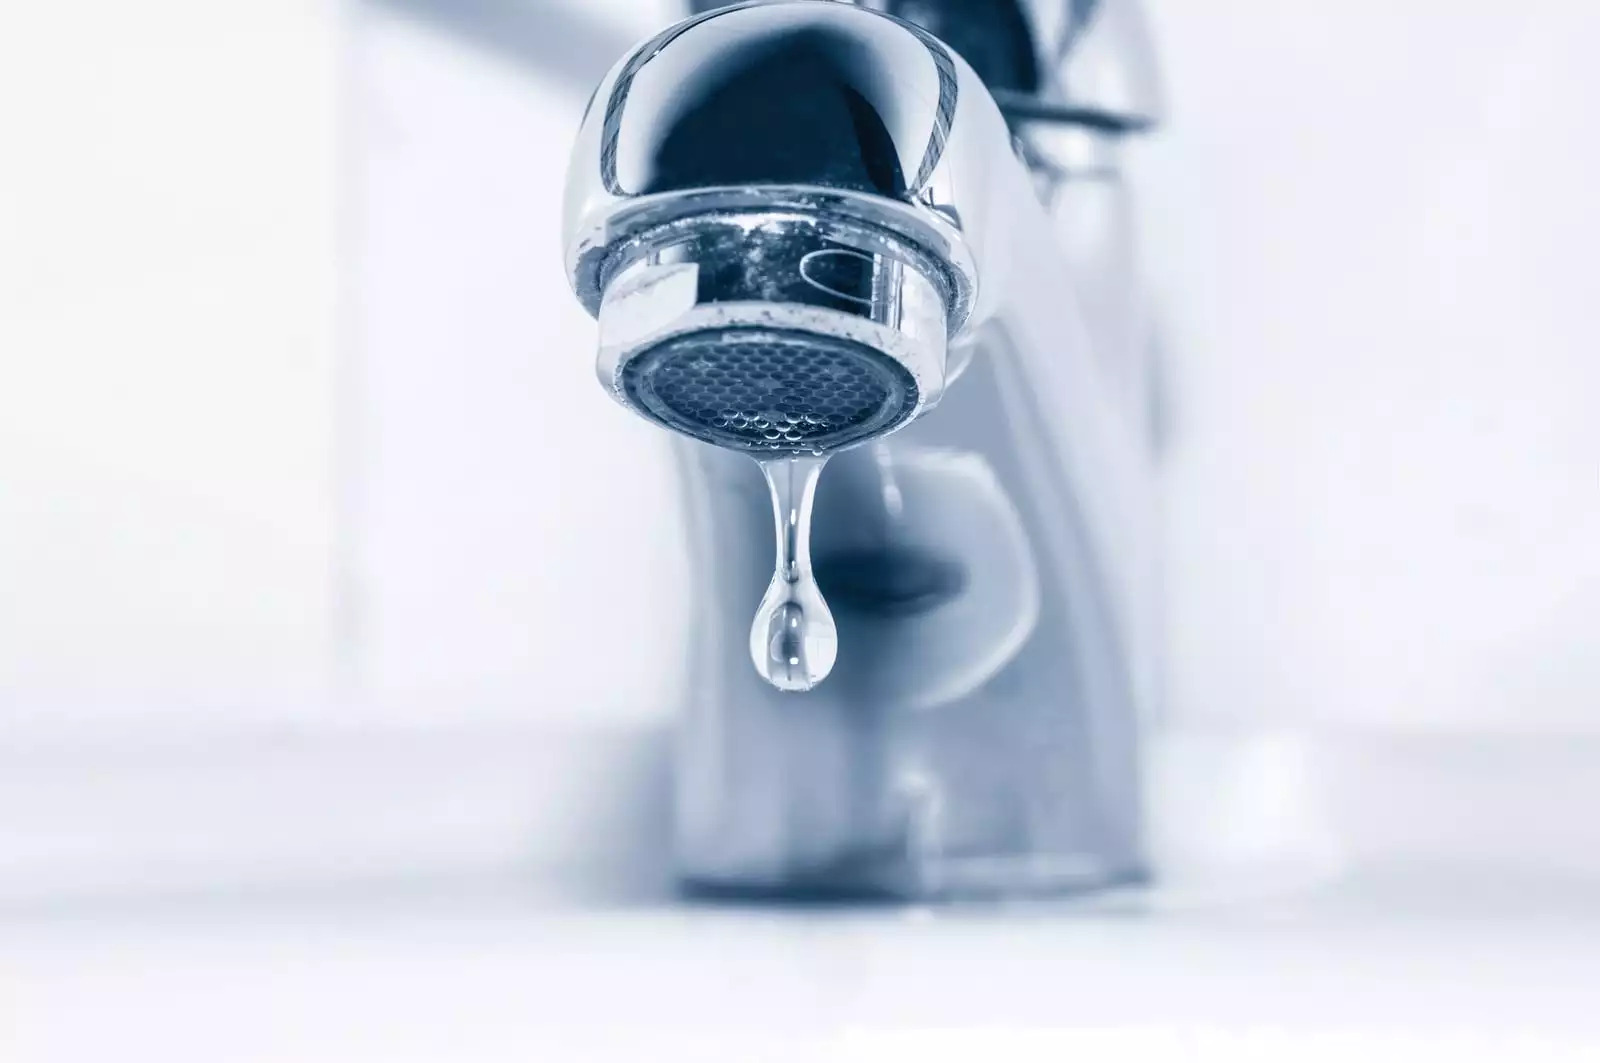
\includegraphics[width=1\textwidth]{img/faucet_1.jpg}
        \end{figure}
    \end{center}
\end{frame}

\begin{frame}
    \begin{figure}
        
    \begin{align*}
    \begin{split}
        \odv{}{t} \left(m \odv{z}{t}\right) &= -kz - \gamma\odv{z}{t} + mg \\
        \odv{m}{t} &= Q,
    \end{split}
    \label{eq:msm_original_odes}
    \end{align*}
    
    \begin{equation*}
        \begin{aligned}
            & k~=
            \begin{cases}
                -11.4\ m + 52.5 \hspace{10mm} (m < 4.61) \\
                \hspace{14.5mm} 0 \hspace{20mm} (m \ge 4.61 )
            \end{cases}
        \end{aligned}
        \label{eq:spring_stiffness}
    \end{equation*}
    
    \begin{equation*}
        z_{\mathrm{c}} = 5.5
        \label{eq:z_critical_model}
    \end{equation*}

    \begin{equation*}
        m_{\mathrm{r}} = 0.2 m + 0.3
    \end{equation*}
    
    \caption{Taken from (Shaw, 1984)}
    \end{figure}
\end{frame}

\begin{frame}
    \begin{center}
        \begin{figure}
            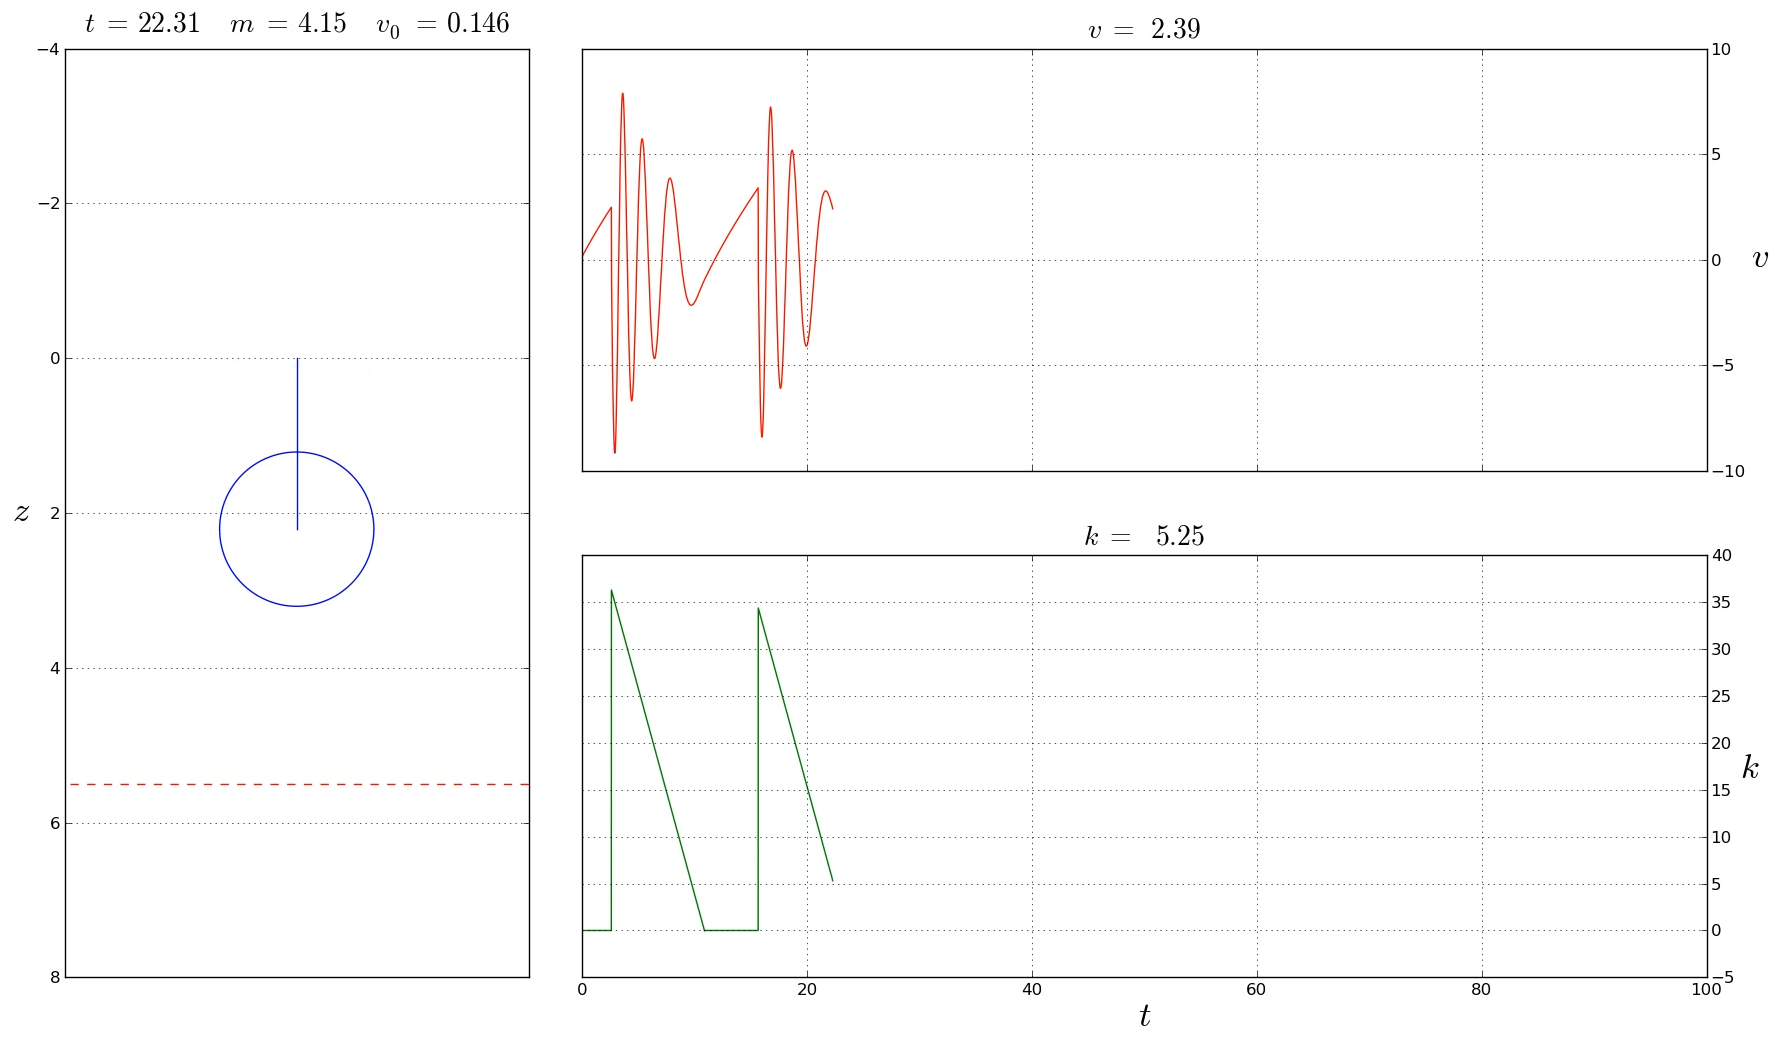
\includegraphics[width=1\textwidth]{./img/msmm_thumbnail.png}
            \caption{Taken from (Nonlinear processes in accretion discs, Květoň, 2014)}
        \end{figure}
    \end{center}
\end{frame}

\begin{frame}
    \begin{center}
        \begin{figure}
            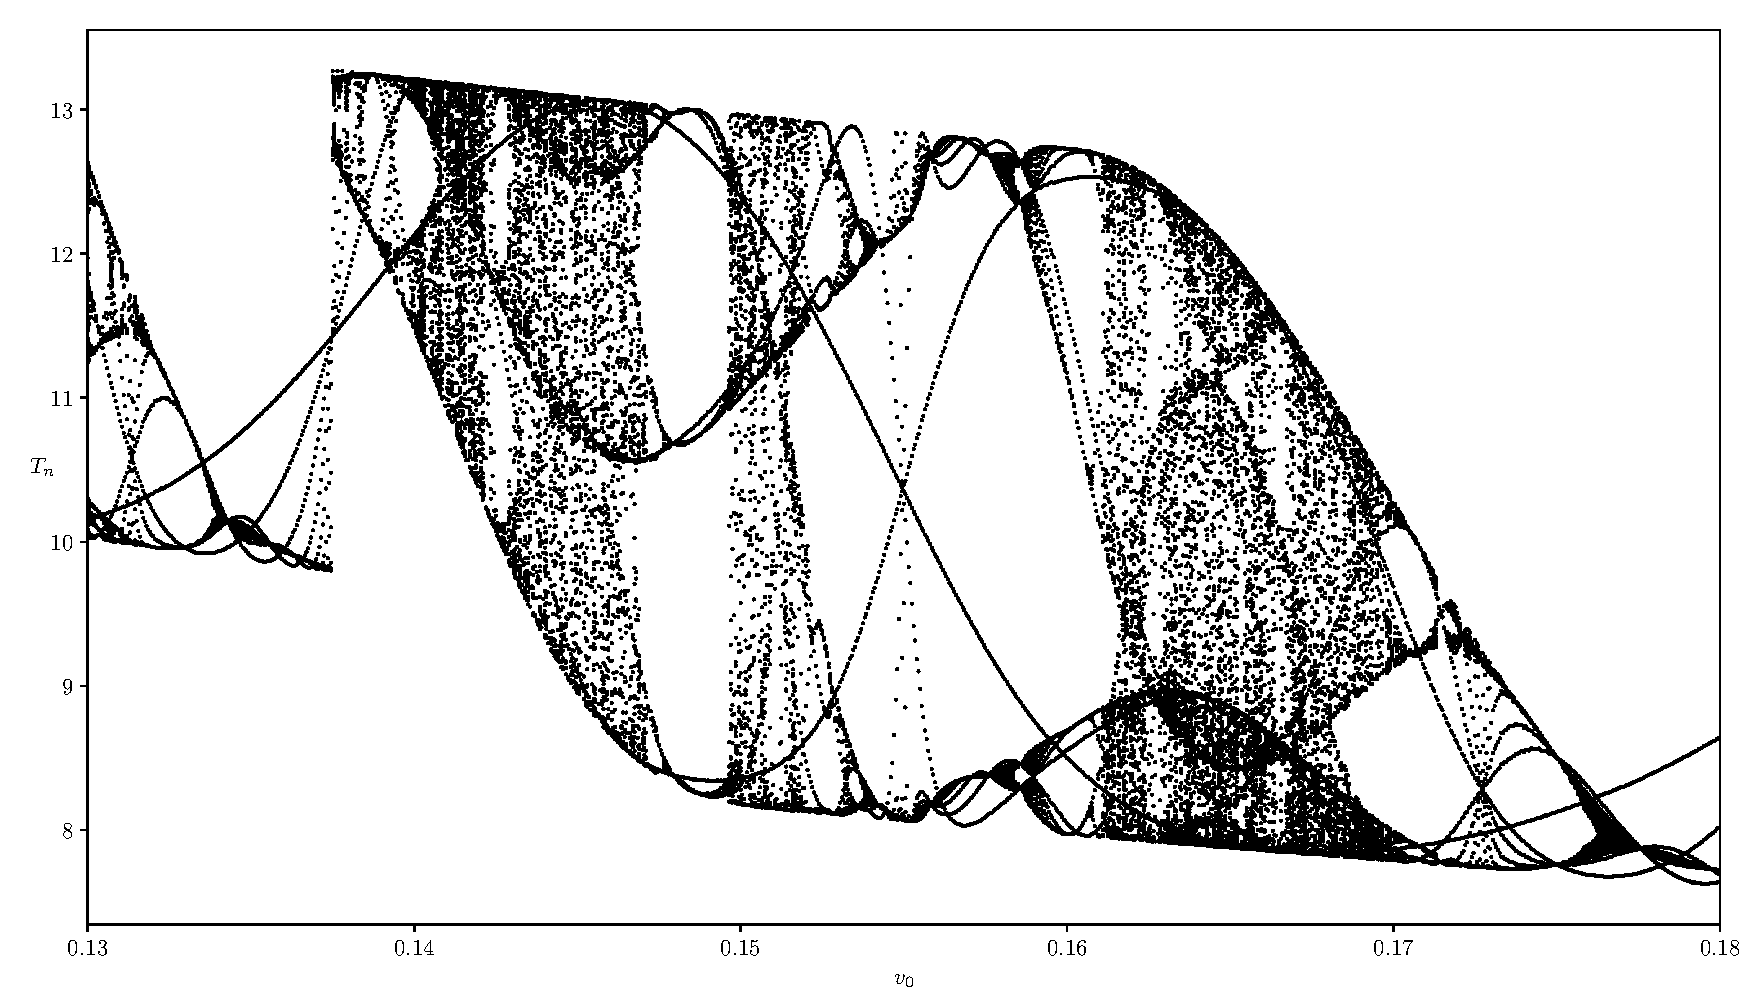
\includegraphics[width=1\textwidth]{../img/plot_msm_bifurcation.pdf}
            \caption{MSM bifurcation diagram}
        \end{figure}
    \end{center}
\end{frame}


%% Vysvětlení modelu
\section{MDH Model}

\begin{frame}
    \begin{center}
        \begin{figure}
            \includegraphics[width=.9\textwidth]{../img/plot_density_temperature_c6.pdf}
            \caption{MDH - C6 simulation snapshot}
        \end{figure}
    \end{center}
\end{frame}

\begin{frame}
    \begin{center}
        \begin{figure}
            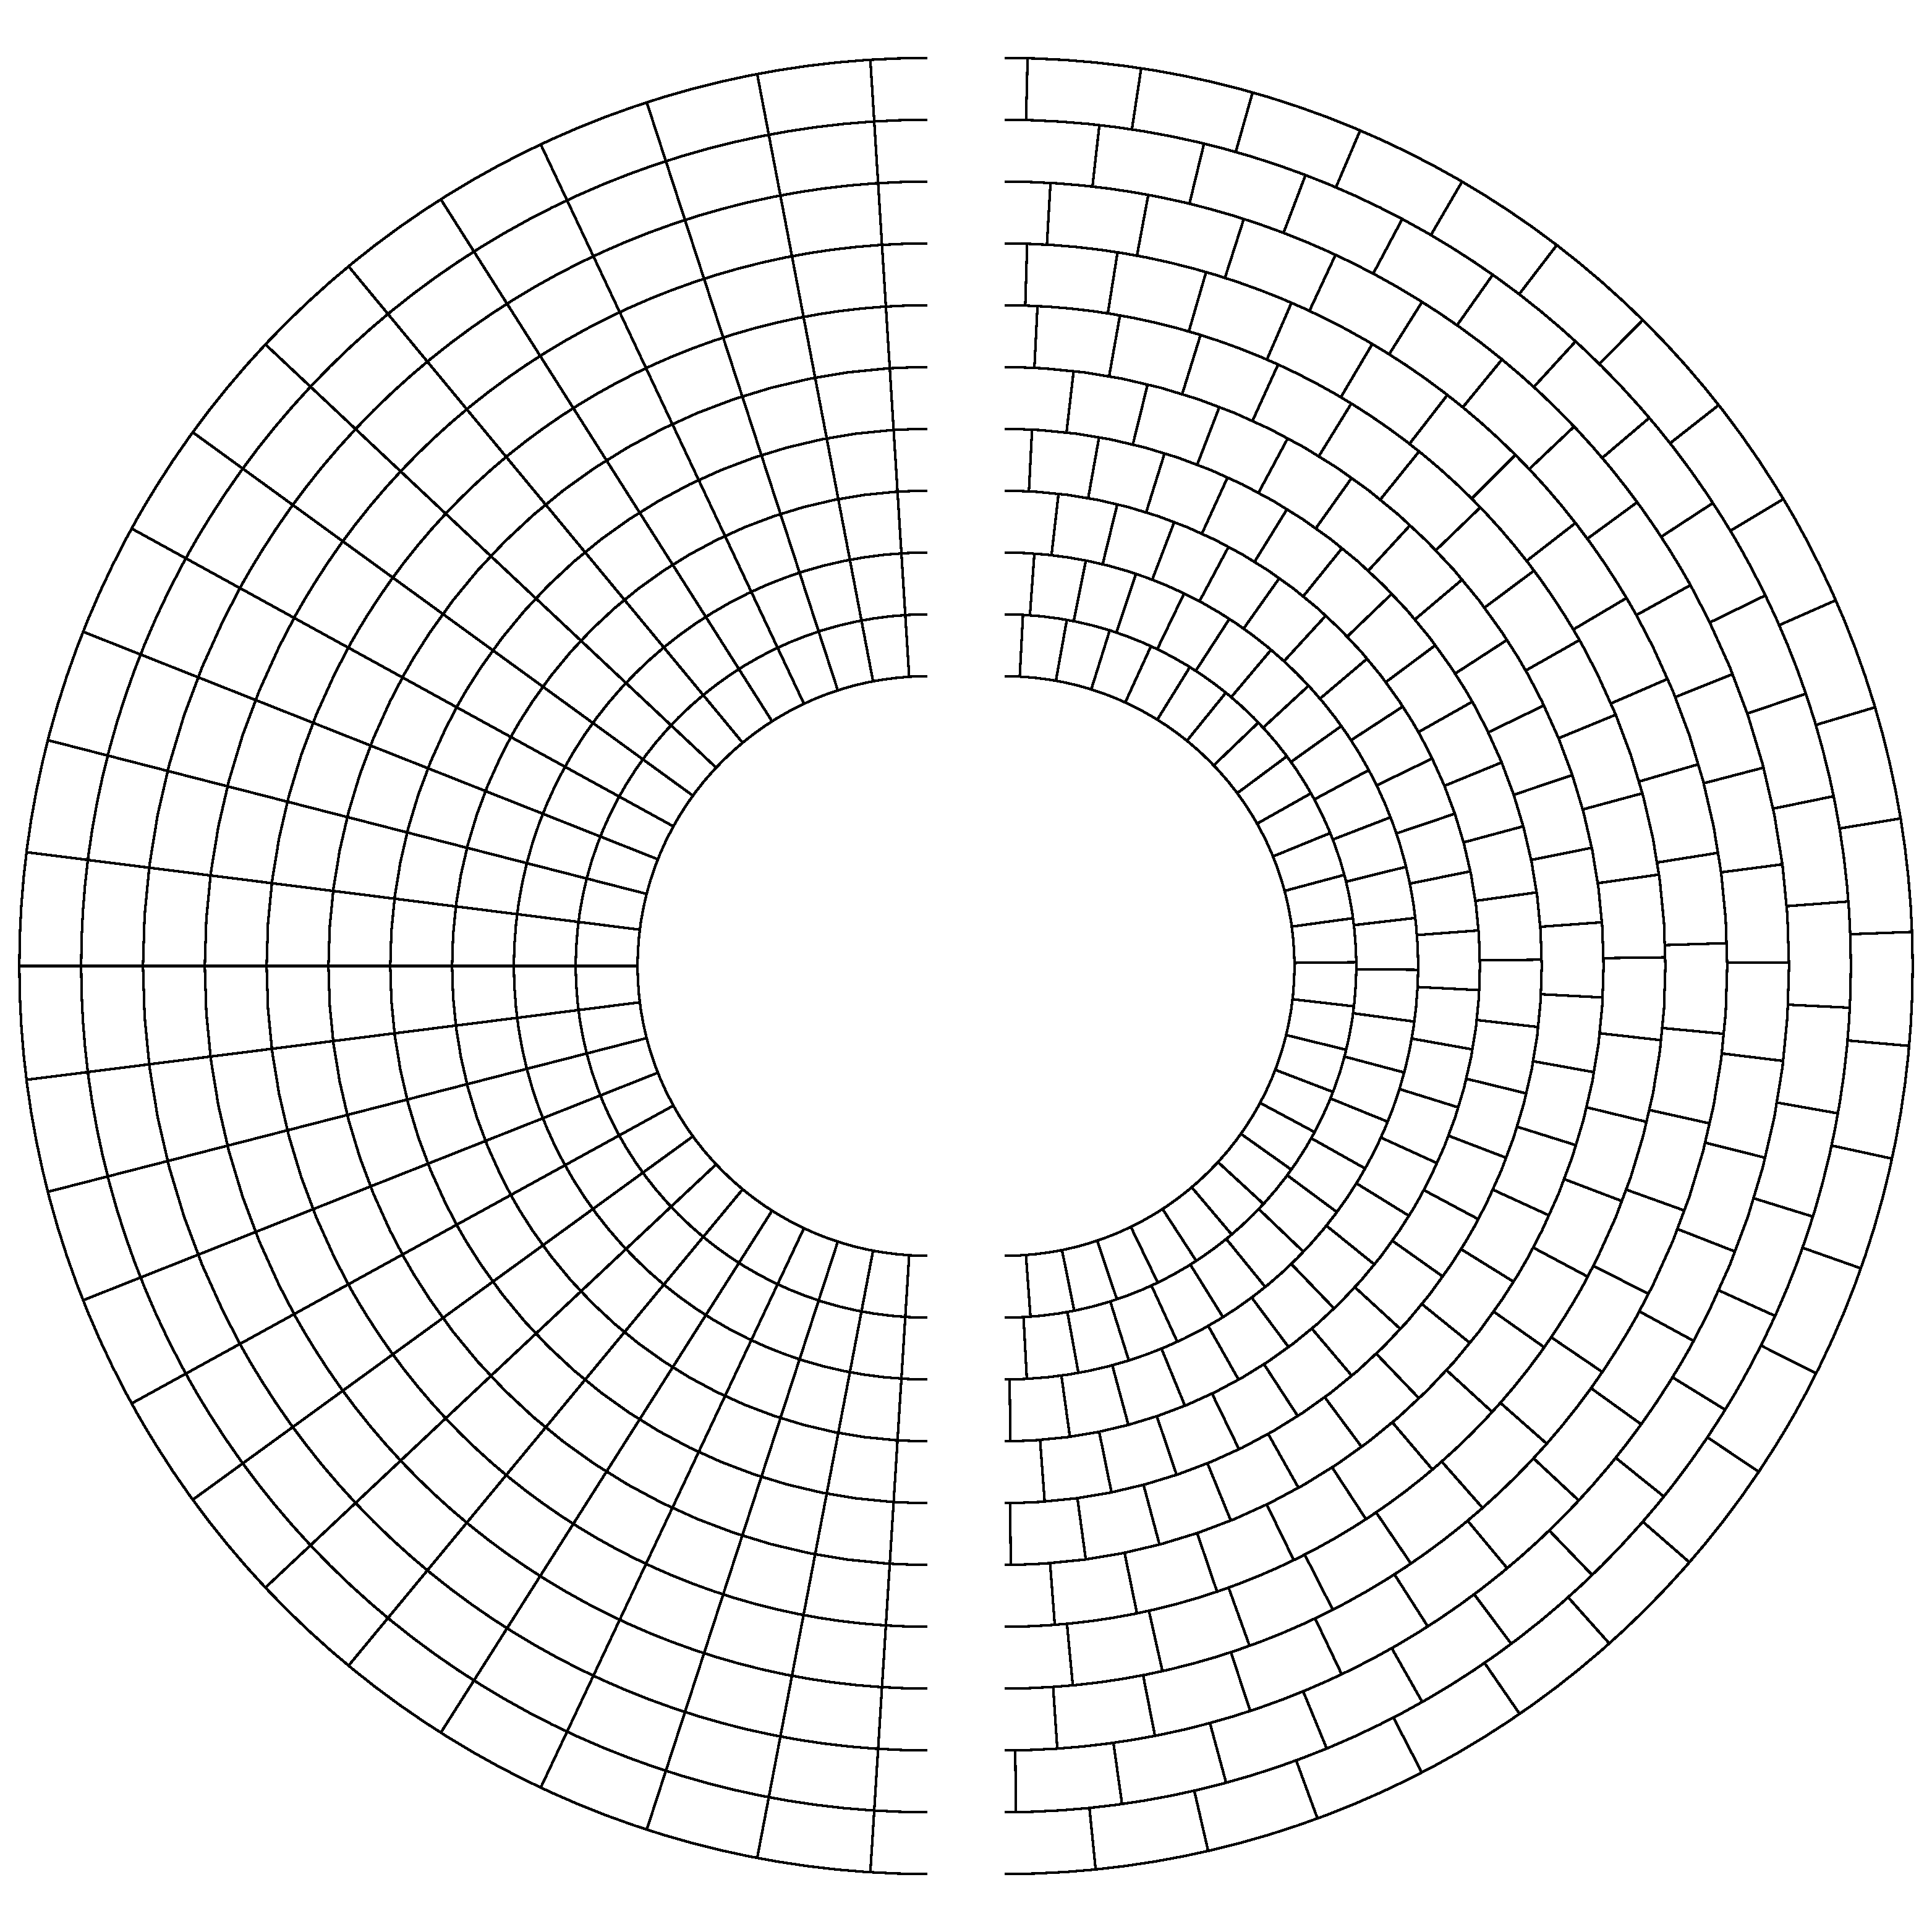
\includegraphics[height=.8\textheight]{../img/grid_states.pdf}
            \caption{Initial grid state (left) and shifted during simulation (right)}
        \end{figure}
    \end{center}
\end{frame}

\begin{frame}
    \begin{center}
        \begin{figure}
            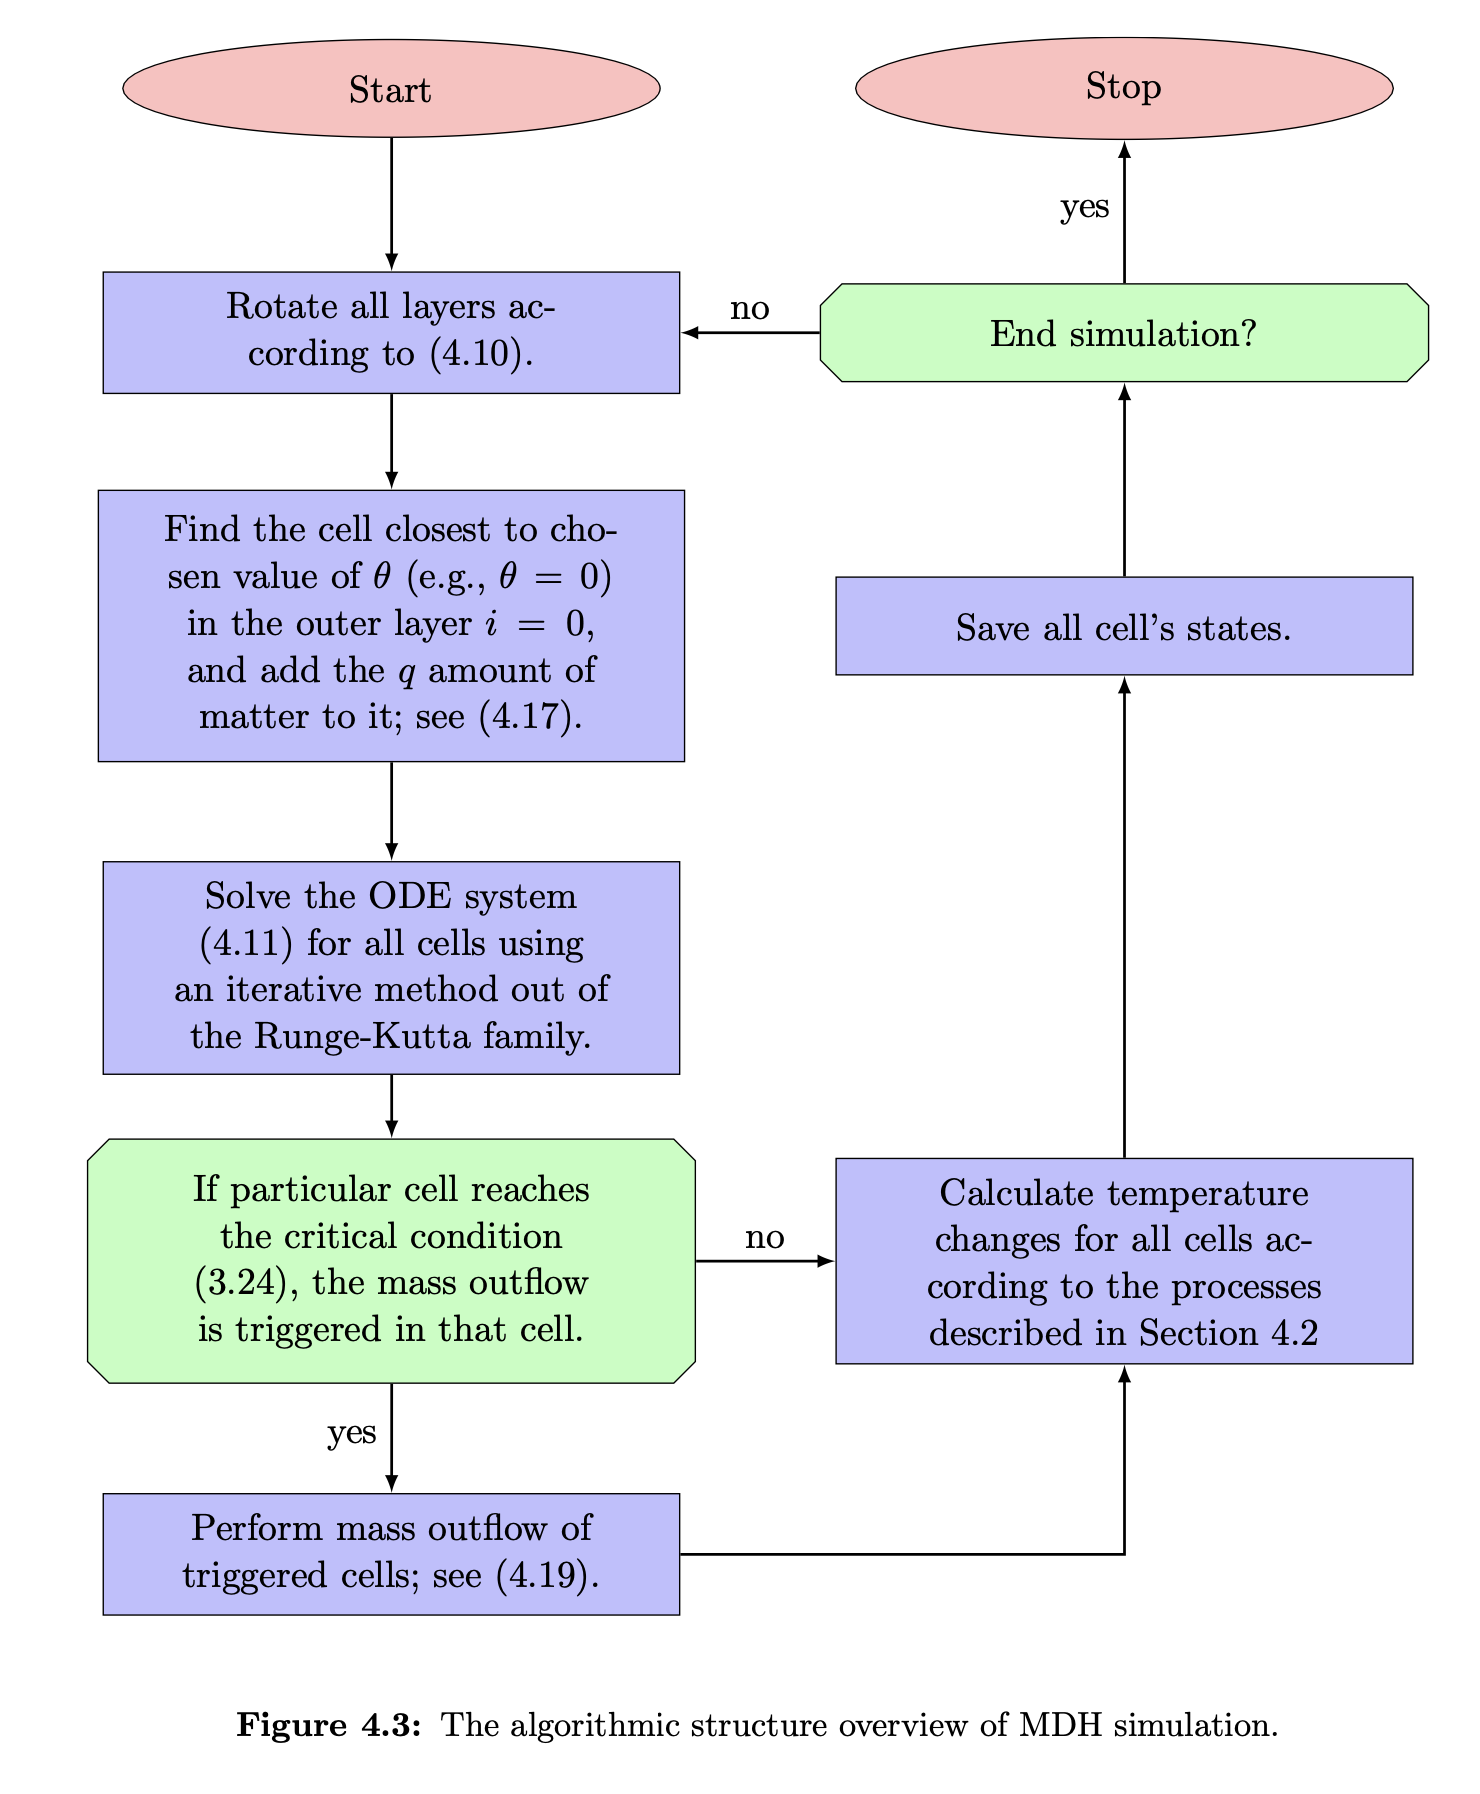
\includegraphics[height=0.9\textheight]{./img/algorithm_1.png}
            % \caption{Taken from (NASA’s Goddard Space Flight Center, 2019)}
        \end{figure}
    \end{center}
\end{frame}

\begin{frame}
    \begin{center}
        \begin{figure}
            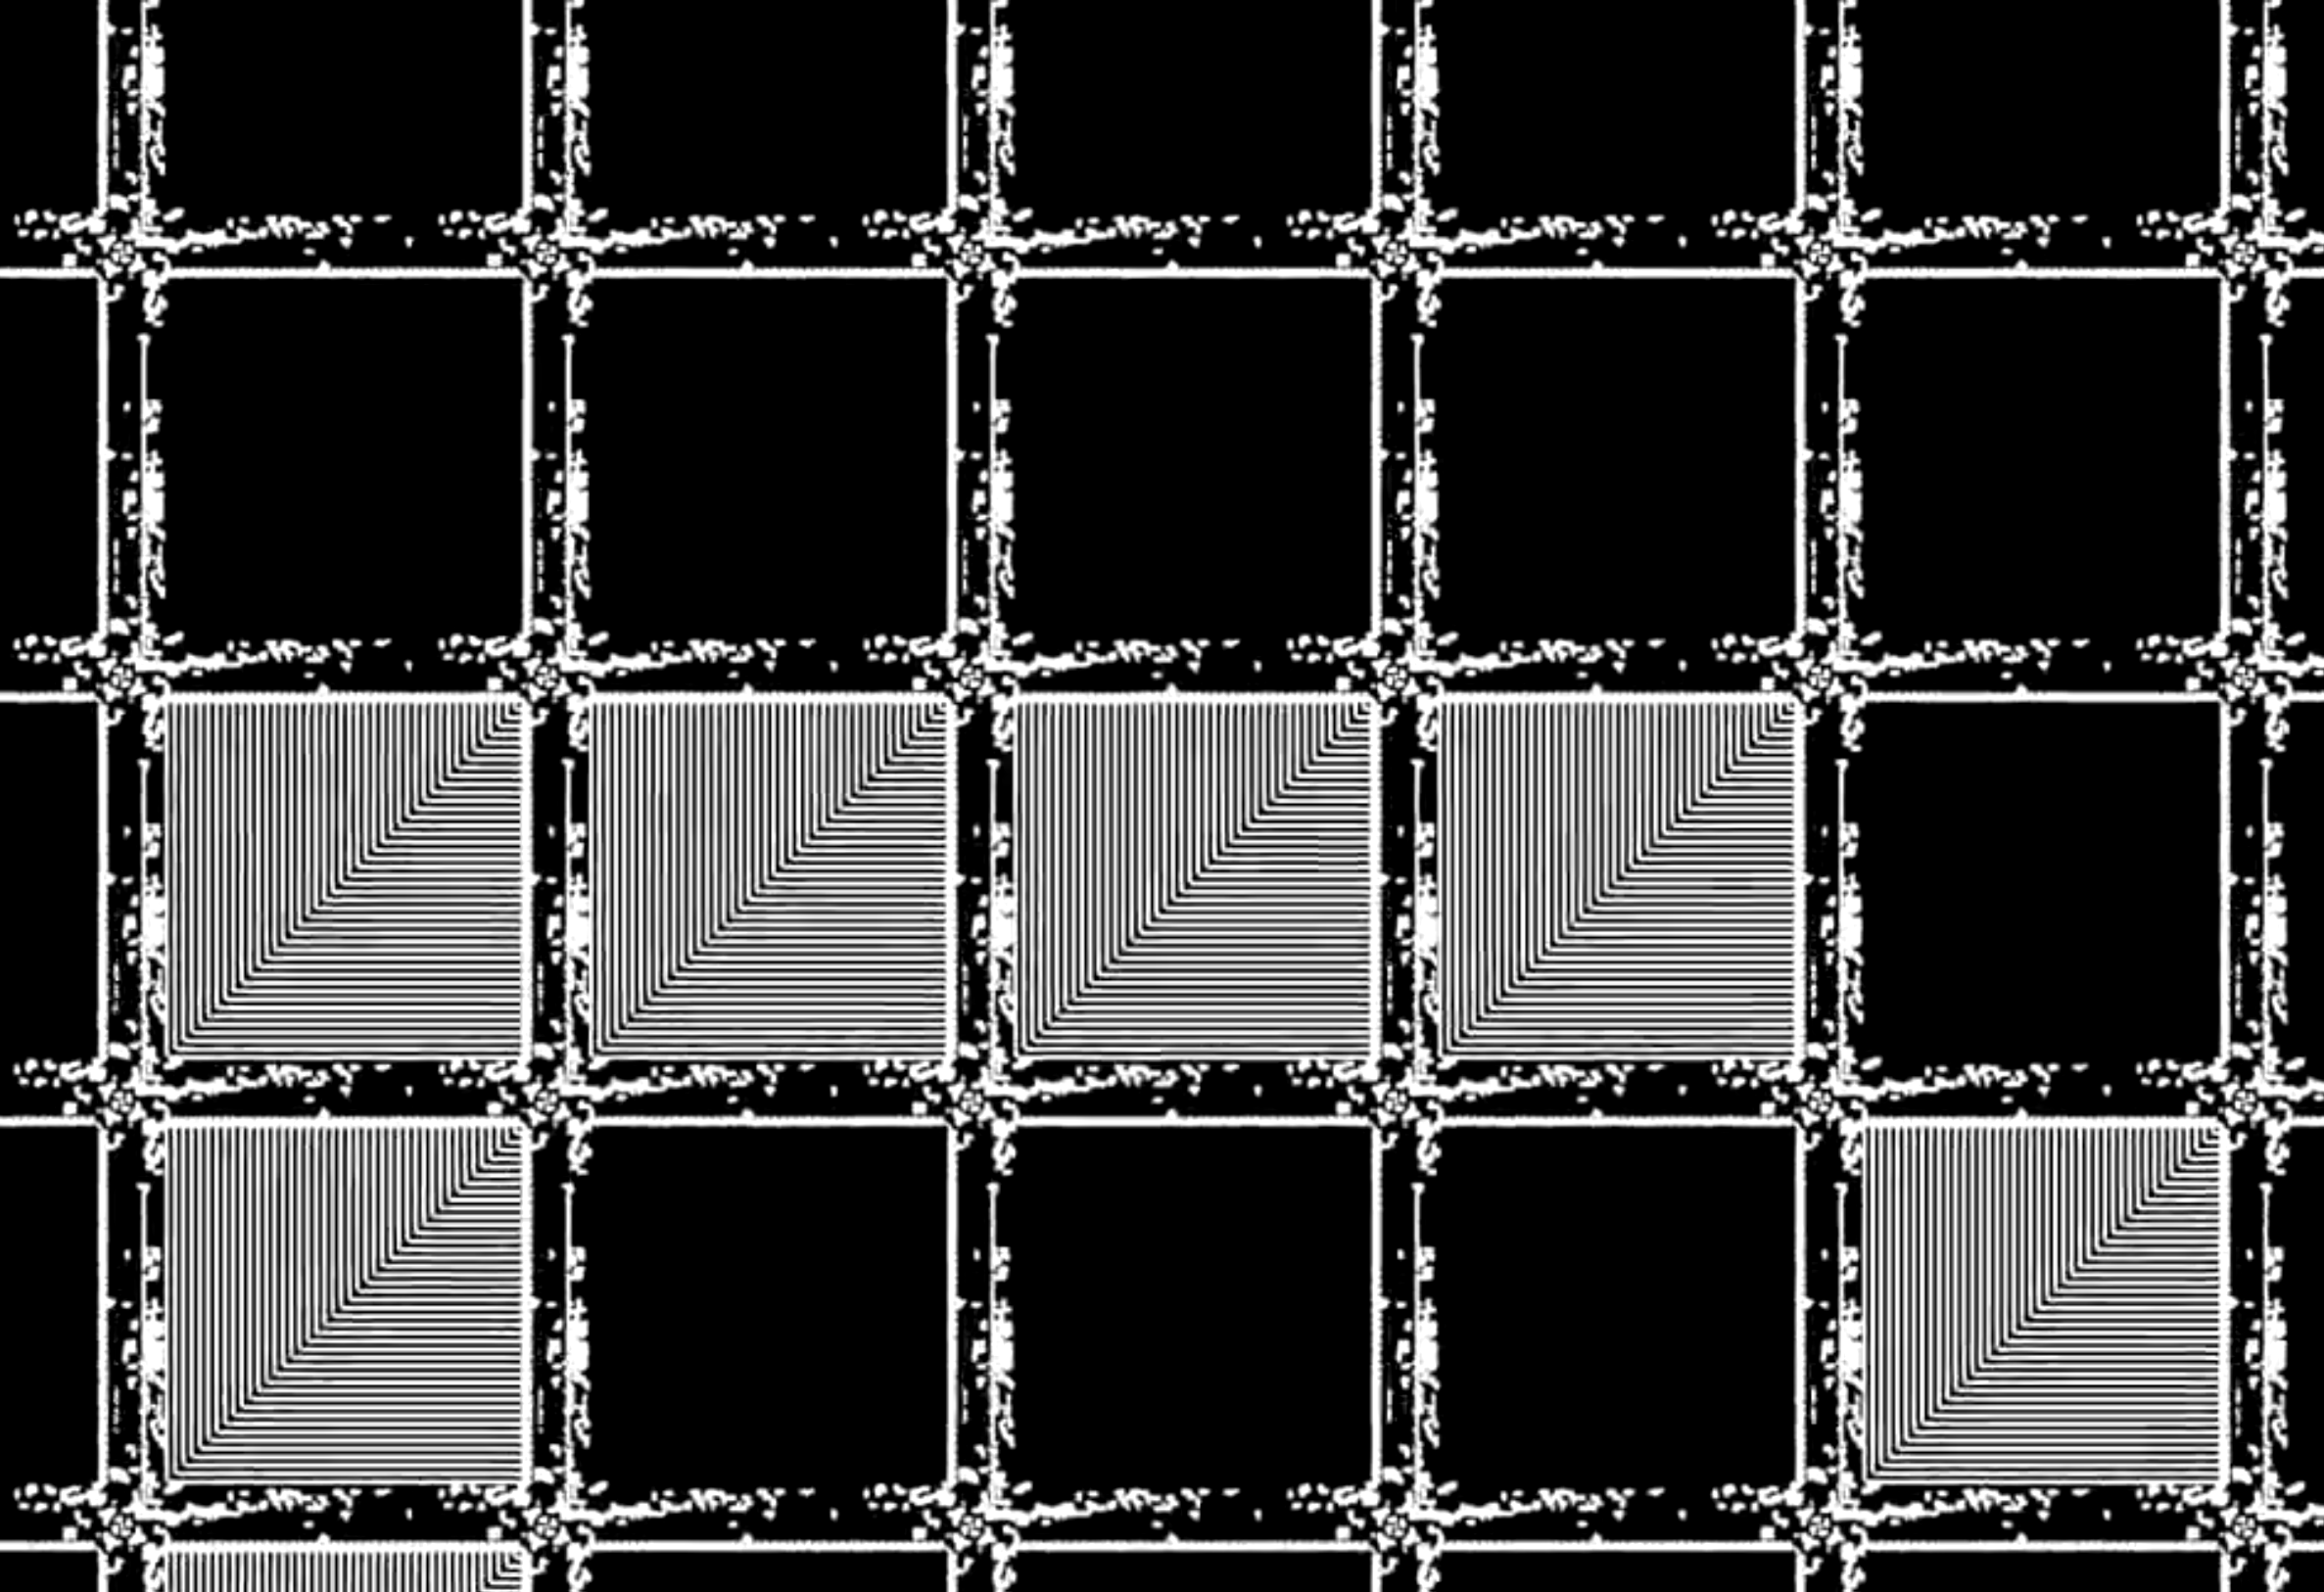
\includegraphics[width=0.9\textwidth]{./img/game_of_live_thumbnail.png}
            \caption{Taken from (Youtube, Philip Bradbury - Life in life, 2012)}
        \end{figure}
    \end{center}
\end{frame}

\begin{frame}
    \begin{figure}
            
        %% free-free emission heating
        \begin{equation*}
            \Delta T_{i+1,j} = \frac{1}{3} \frac{G M_{\mathrm{p}} \Delta m_{ij} \Delta r}{r_{i}^2 \mathcal{R} m_{i+1,j}}
            \label{eq:temp_ff_final}
        \end{equation*}

        % gas mixing
        \begin{equation*}
        T_{i+1,j}' = \frac{m_{i+1,j} T_{i+1,j} + \Delta m_{ij} T_{ij}}{m_{i+1,j} + \Delta m_{ij}}
        \end{equation*}

        % radiative cooling
        \begin{equation*}
        T_{ij}' = \left( \frac{2 \sigma S_{ij} t}{m_{ij} \mathcal{R}} + \frac{1}{T_{ij}^3} \right)^{-1/3}
        \end{equation*}

        % t_out
        \begin{equation*}
        T_{\mathrm{out}} \sim 10^3\, \mathrm{K}
        \end{equation*}

        \caption{Thermal processes definition based on (Yonehara et al., 1997)}
    \end{figure}
\end{frame}

\begin{frame}
    \begin{equation*}
        L_{\lambda,ij} = 4\pi \cdot S_{ij} \cdot B_{\lambda,ij}(\lambda, T_{ij})
        \label{eq:facet_radiation}
    \end{equation*}

    \bigskip

    \begin{equation*}
    L_{\mathrm{F}} = 4 \pi S_{ij} \Delta \lambda \sum_{i=0}^{I-1} \sum_{j=0}^{J-1} \sum_{\lambda=0}^{\infty} B_{\lambda,ij}(\lambda, T_{ij})\,g(\lambda)
    \end{equation*}
\end{frame}

\begin{frame}
    \begin{equation*}
    g(\lambda) \propto \mathrm{exp}\left[ - \frac{1}{2} \left( \frac{\lambda - \lambda_{\mathrm{c}}}{\lambda_{\mathrm{w}}} \right)^2 \right]
    \label{eq:filter_gauss}
    \end{equation*}

    \bigskip

    \begin{center}
        \begin{figure}
            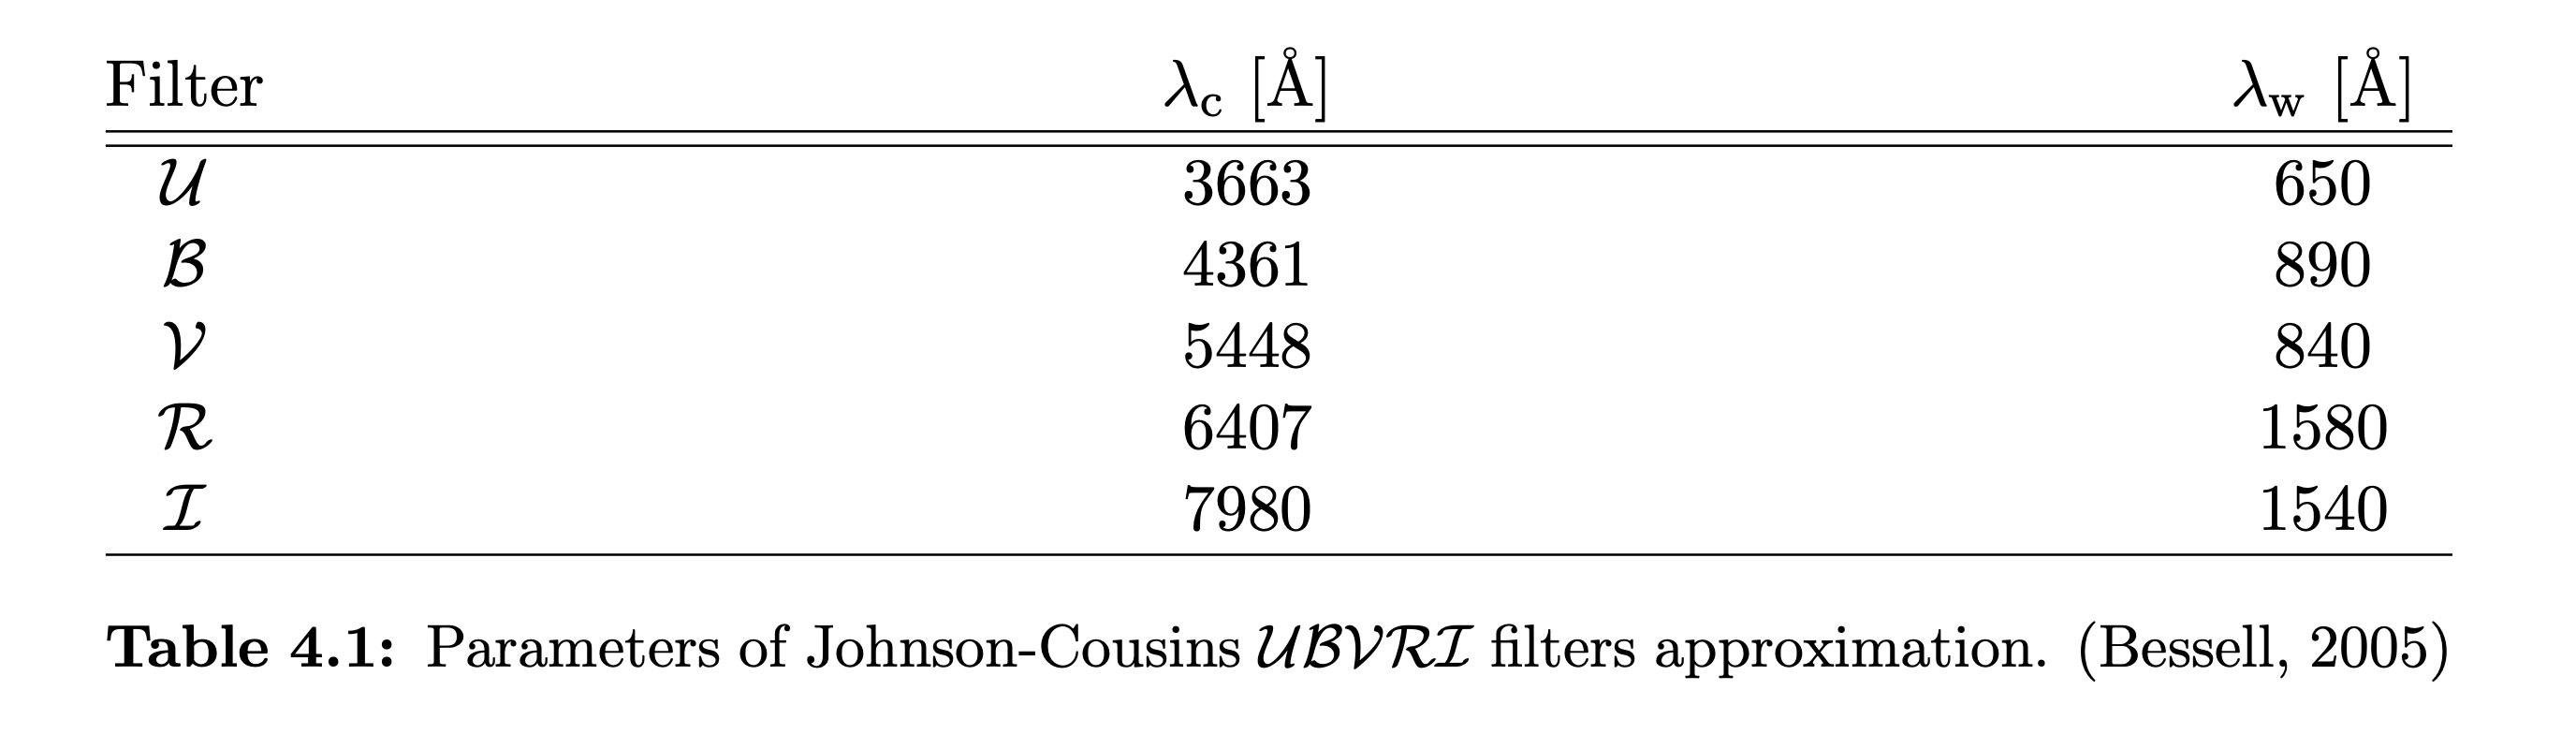
\includegraphics[width=.95\textwidth]{./img/filter_table.png}
            % \caption{Taken from (NASA’s Goddard Space Flight Center, 2019)}
        \end{figure}
    \end{center}
\end{frame}



%% Implementace
\section{Implementation}
\begin{frame}
    \large
    \begin{center}
        \textbf{Initial requirements}
    \end{center}
    \bigskip
    \begin{itemize}
        \item{Solve a large number of ODE sets (individual MSM models)}
        \bigskip
        \bigskip
        \item{Handle a large amout of data output (in order of TB per simulation)}
    \end{itemize}
\end{frame}

\begin{frame}
    \begin{center}
    \begin{tabular}{ll}
        
\includegraphics[width=.3\linewidth,valign=m]{./img/cpp_logo.com.png} & 
\includegraphics[width=.3\linewidth,valign=m]{./img/Open_MPI_logo.png}\\
        
\includegraphics[width=.3\linewidth,valign=m]{./img/python_logo.png} & 
\includegraphics[width=.3\linewidth,valign=m]{./img/HDF_transparent_original.png}\\
    \end{tabular}
    \end{center}
\end{frame}

\begin{frame}
    \begin{itemize}
        \item{\textbf{SIMULATION} (SIM) - Performs the dynamical simulation of matter flow and temperature changes in the accretion disc.}
        \bigskip
        \item{\textbf{RADIATION} (RAD) - Takes the dynamical simulation results and com- putes the disc’s power output spectral distribution over the predefined range of wavelengths.}
        \bigskip
        \item{\textbf{OBSERVATION} (OBS) - Performs a synthetic observation, with the use of analytical approximations of Johnson-Cousins UBVRI photometric filters, and extracts a flickering light curve.}
    \end{itemize}
\end{frame}

%% Video ukázky
\section{Results}
\begin{frame}
    \begin{center}
        \begin{figure}
            \includegraphics[width=.9\textwidth]{../img/plot_density_temperature_c7.pdf}
            \caption{MDH - C7 simulation snapshot}
        \end{figure}
    \end{center}
\end{frame}

\begin{frame}
    \begin{center}
        \begin{figure}
            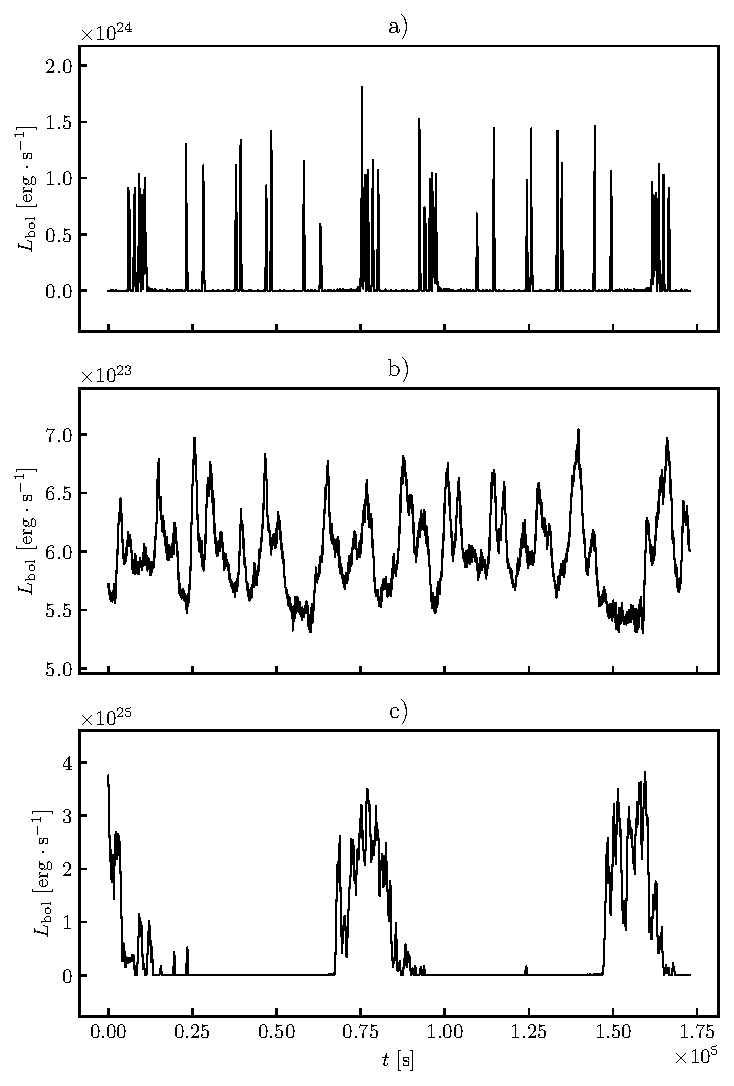
\includegraphics[height=.9\textheight]{../img/plot_light_curves_undisturbed.pdf}
            \caption{Synthetic light curves - a) \textbf{C2} b) \textbf{C3} c) \textbf{C4}}
        \end{figure}
    \end{center}
\end{frame}

\begin{frame}
    \begin{center}
        \begin{figure}
            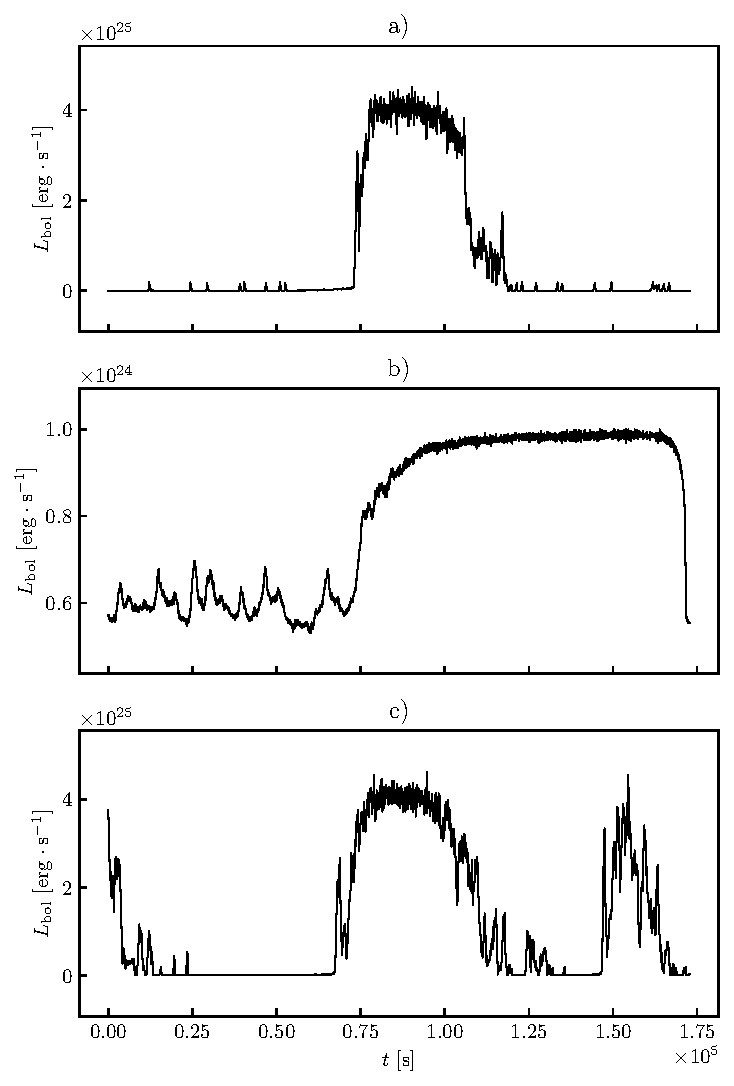
\includegraphics[height=.9\textheight]{../img/plot_light_curves_disturbed.pdf}
            \caption{Synthetic light curves - a) \textbf{C5} b) \textbf{C6} c) \textbf{C7}}
        \end{figure}
    \end{center}
\end{frame}

%% alpha parametr fitting
\section{Shakura-Sunyaev $\alpha-$model fitting}
\begin{frame}
    \footnotesize
    \begin{figure}
        \begin{align*}
            \begin{split}
                \Sigma &= 5.2 \alpha^{-4/5} \dot{M}^{7/10}_{16} m^{1/4}_1 R^{-3/4}_{10} f^{14/5}\ \mathrm{g\ cm^{-2}} \\
                H &= 1.7 \times 10^8 \alpha^{-1/10} \dot{M}^{3/20}_{16} m^{-3/8}_1 R^{9/8}_{10} f^{3/5}\ \mathrm{cm} \\
                \rho &= 3.1 \times 10^{-8} \alpha^{-7/10} \dot{M}^{11/20}_{16} m^{5/8}_1 R^{-15/8}_{10} f^{11/5}\ \mathrm{g\ cm^{-3}} \\
                T_{\mathrm{c}} &= 1.4 \times 10^4 \alpha^{-1/5} \dot{M}^{3/10}_{16} m^{1/4}_1 R^{-3/4}_{10} f^{6/5}\ \mathrm{K} \\
                \tau &= 190 \alpha^{-4/5} \dot{M}^{1/5}_{16} f^{4/5} \\
                \nu	&= 1.8 \times 10^{14} \alpha^{4/5} \dot{M}^{3/10}_{16} m^{3/4}_1 R^{3/4}_{10} f^{6/5}\ \mathrm{cm^2\ s^{-1}}  \\
                v_{\mathrm{R}}	&= 2.7 \times 10^{14} \alpha^{4/5} \dot{M}^{3/10}_{16} m^{-1/4}_1 R^{-1/4}_{10} f^{-14/15}\ \mathrm{cm\ s^{-1}}  \\
                \mathrm{with}\ f &= \left[ 1 - \left( \frac{R_*}{R} \right)^{1/2} \right]^{1/4} \\
            \end{split}
        \end{align*}
        \caption{Shakura-Sunyaev $\alpha-$disc model solution (Frank et al., 2002)}
    \end{figure}

\end{frame}

\begin{frame}
    \normalsize
    \begin{center}
        \begin{figure}
            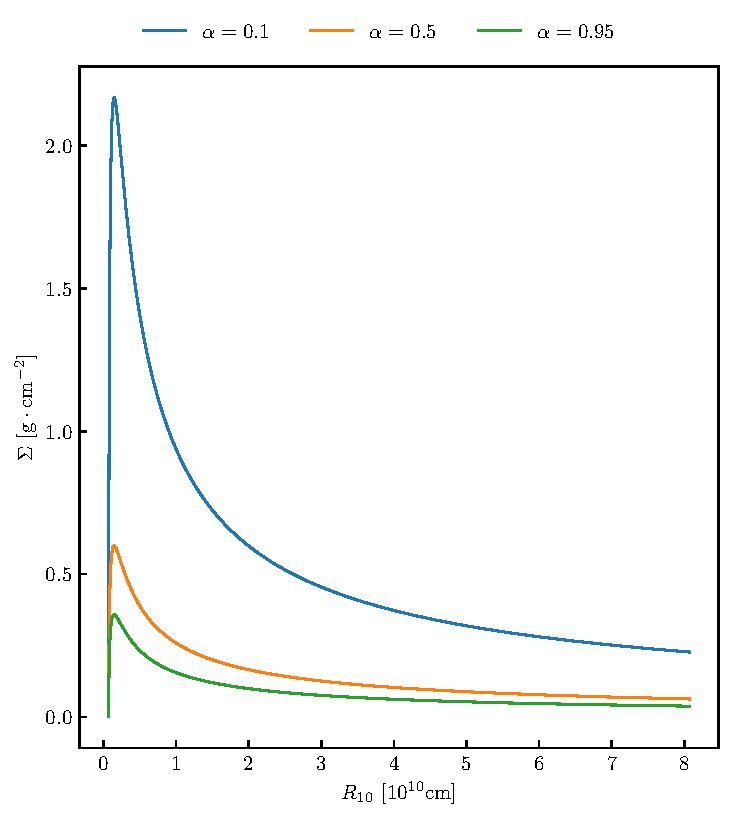
\includegraphics[height=.85\textheight]{../img/plot_density_analytical.pdf}
            \caption{Examples of Shakura-Sunyaev $\alpha-$disc area density solution}
        \end{figure}
    \end{center}
\end{frame}

\begin{frame}
    \begin{center}
        \begin{figure}
            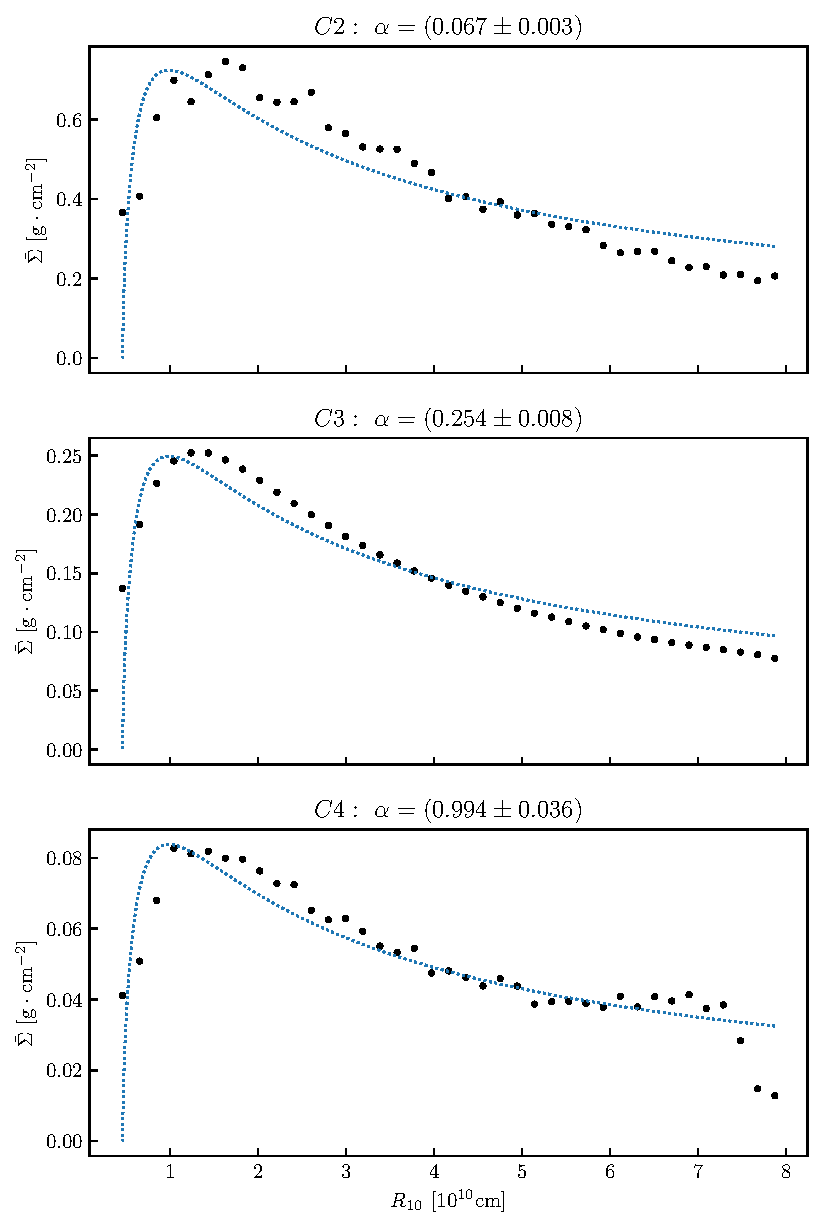
\includegraphics[height=.85\textheight]{../img/plot_mean_density_fit.pdf}
            \caption{Examples of Shakura-Sunyaev $\alpha-$parameter fits for mean area density}
        \end{figure}
    \end{center}
\end{frame}

\begin{frame}
    \begin{center}
        \begin{figure}
            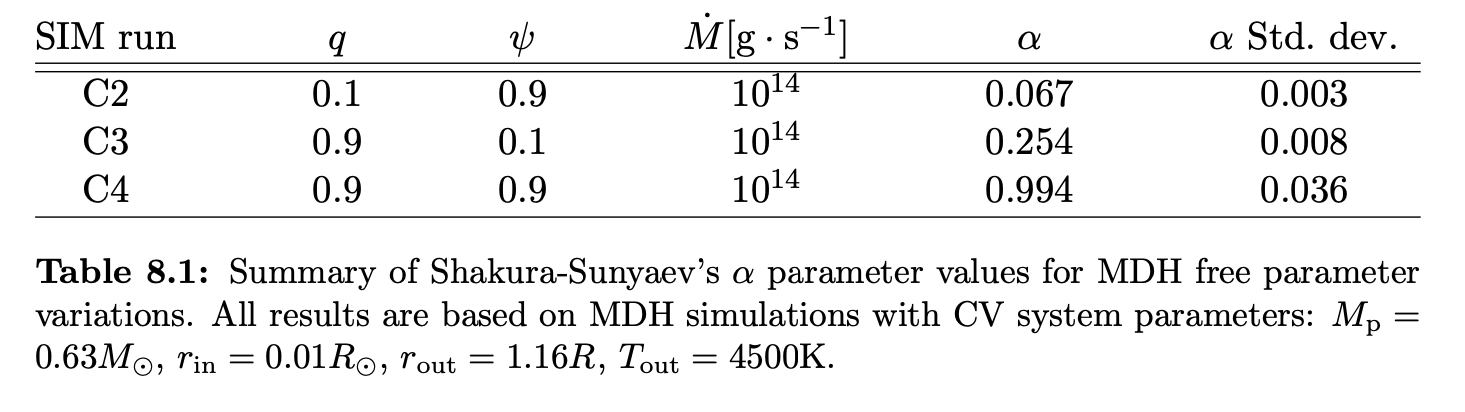
\includegraphics[width=.9\textwidth]{./img/table_alpha_results.png}
            % \caption{Examples of Shakura-Sunyaev $\alpha-$parameter fits for mean area density}
        \end{figure}
    \end{center}
\end{frame}


%% Diskuze
\section{Discussion}
\begin{frame}
    \Huge
    \begin{figure}
        \begin{center}
            -- Thank you -- 
        \end{center}
    \end{figure}
\end{frame}


\end{document}
